\section{Begriffliche Grundlagen}

\textbf{Deduktion} (logisches Schließen): Vom Allgemeinen aufs Spezifische schließen \textit{(von generellen Axiomen auf spezielle Theoreme schließen)}.\\[5pt]
\textbf{Induktion} (Lernen durch Generalisierung von Beispielen): Vom Spezifischen aufs Allgemeine schließen \textit{(von speziellen Beispielen auf generelle Regeln, Theorien schließen)}.\vspace*{-5pt}
\begin{itemize}[$\hookrightarrow$]
	\leftskip10pt
	\item Schlussfolgerung über die Validität einer Theorie basiert auf Erfahrung
	\item Theorien sind nie \dq wahr\dq oder \dq existent\dq
	\item Theorien können falsifiziert werden, aber nicht verifiziert
	\item Theorien können nur durch Beobachtungen gestützt werden
\end{itemize}
\textbf{Abduktion}: Schließen ausgehend von Beispielen anhand von Regeln. Von einem speziellen Beispiel wird durch Rückwärtsanwendung von bekannten Regeln versucht daraus zu schließen (kann logisch richtig zu falschen Schlüssen führen).
\begin{figure}[ht]
	\centering
	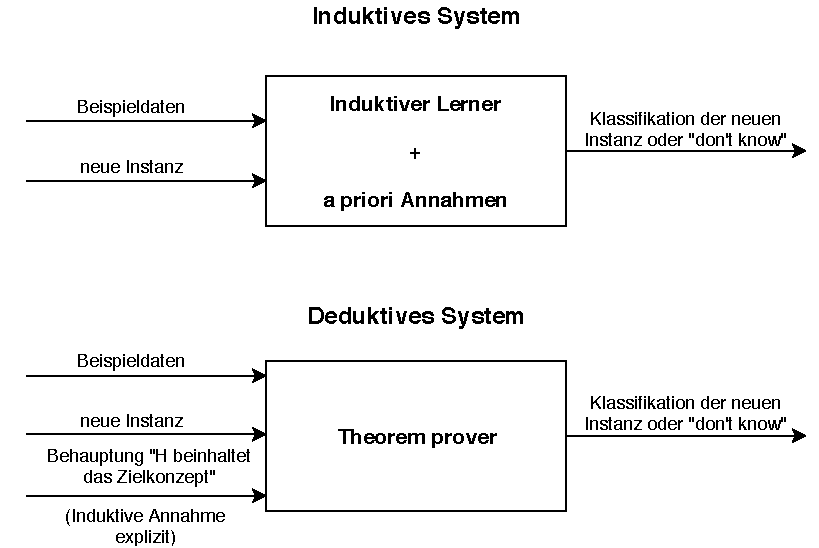
\includegraphics[width=.85\textwidth]{img/inductiveSystem}
	\caption{Induktives Lernen und äquivalentes deduktives System}
	\label{deployment}
\end{figure}\\
\textbf{Generalisierung} (generalization): Gelerntes Modell auf neue Eingaben (die nicht zum Lernen benutzt wurden) anwenden.\\[5pt]
\textbf{Feature extraction}: Eingabedaten werden Vorverarbeitet (pre-processing) damit das Problem einfacher wird (auch um Zeit-/Platzkomplexität zu reduzieren).\vspace*{-5pt}
\begin{itemize}[$\hookrightarrow$]
	\leftskip10pt
	\item Dimensionsreduktion
	\item Informationsverlust
\end{itemize}	
\textbf{Klassifikation} (classification): Jede Eingabe wird einer endlichen Anzahl von diskreten Kategorien zugewiesen.\\[5pt]
\textbf{Regression} (regression): Jede Eingabe wird einer oder mehreren (Vektor) stetigen Variablen zugewiesen.\\[5pt]
\textbf{Eingaben} (inputs): Menge von Eingaben $X = \{x_1, ... , x_n\}$ zu einer Funktion.\\[5pt]
\textbf{Ausgaben} (targets): Menge von Sollausgaben $T=\{t_1, ..., t_n\}$. zu einer Funktion.\\[5pt]
\textbf{Trainingsdaten} (training set): Große Menge von Eingabedaten $X = \{x_1, ... , x_n\}$, manchmal mit den zugehörigen Sollausgaben $T=\{t_1, ..., t_n\}$.\\[5pt]
\textbf{Lineare Modelle} (linear models): Funktionen, die linear in den unbekannten Parametern sind.\\[5pt]
\textbf{Inductive learning hypothesis}: Jede Hypothese, die die Zielfunktion gut über eine ausreichend große Anzahl an Trainingsdaten approximiert, approximiert die Zielfunktion auch gut über neue Daten.\vspace*{-5pt}
\begin{itemize}[$\hookrightarrow$]
	\leftskip10pt
	\item Daten sind charakteristisch für generelle Regel/Funktion
	\item ist immer eine implizite Annahme
\end{itemize}
\textbf{Learning bias}: Bezeichnet die impliziten Annahmen über die Art der Generalisierung.\vspace*{-5pt}
\begin{itemize}[$\hookrightarrow$]
	\leftskip10pt
	\item ist immer notwendig!
\end{itemize}
\textbf{Modellselektion} (model selection): Auswahl einer parametrisierte Form des (Daten-) Modells.\\[5pt]
\textbf{Parameteroptimierung} (parameter optimisation, learning): Optimiere (lerne) die Parameter eines ausgewählten Modells anhand der Trainingsdaten.
